%%%%%%%%%%%%%%%%%  Debut du fichier Latex  %%%%%%%%%%%%%%%%%%%%%%%%%%%%%%
\documentclass[
    a4paper, 
    12pt, onecolumn,
    %draft
]{article}

%%% Pour un texte en francais
\usepackage[francais]{babel}
\usepackage[latin1]{inputenc}	         % encodage des lettres accentuees
\usepackage{graphicx} \def\BIB{}
\usepackage{url}

\usepackage[textwidth=17mm]{todonotes}
\newcommand{\customtodo}[4]{
        \todo[color=#2,inline,size=\small]{
                \ifx&#3&
                        \textbf{#1} #4
                \else
                        \textbf{#1$\Rightarrow$#3} #4
                \fi
        }
}
\newcommand{\HC}[2][]{\customtodo{HC}{red!20}{#1}{#2}}
\newcommand{\IF}[2][]{\customtodo{IF}{blue!20}{#1}{#2}}

\newcommand{\ie}[0]{{\em i.e.},\xspace}
\newcommand{\vs}[0]{{\em vs.}\xspace}
\newcommand{\eg}[0]{{\em e.g.},\xspace}
\newcommand{\etal}[0]{{\em et al.}\xspace}
\newcommand{\wrt}[0]{{\em w.r.t.}\xspace}
\newcommand{\aka}[0]{{\em a.k.a.}\xspace}
\newcommand{\via}[0]{{\em via}\xspace}

%--------------------------------------------------------

\title{Fog-RAN placement problem}
\author{H�l�ne Coullon (Inria, IMT) and Ilhem Fajjari (Orange)}

\begin{document}

\maketitle

%---------------------------------------------------------
\section{From RAN to Cloud-RAN to Fog-RAN}
%---------------------------------------------------------
\IF{Ilhem, add your comments by using this command}
\HC{Helene, add your comments by using this command}

A Radio Access Network (RAN) is a part of a mobile telecommunication system. RAN resides between a mobile device (such as mobile phones or tablets) and the core network (CN)~\footnote{\url{https://en.wikipedia.org/wiki/Radio_access_network}}.

Distributed RAN~\footnote{\url{https://en.wikipedia.org/wiki/C-RAN}} architecture has been introduced for the 3G technology. Unless 1G and 2G architectures, where base stations were responsible for all signal computations, for 3G a distributed base station architecture has been introduced by Nokia, Huawei etc. In this architecture the radio function unit, or Remote Radio Head (RRH) is separated from the baseband unit (or BBU) by a fronthaul network (fiber), which results in lighter base stations that can be placed directly close to antennas, thus reducing signal loss.

The major difficulty of this system is to perfectly choose the size of BBUs pool. In pratice, these pools are designed to answer a very high load onto the network which results in an under-use of the pool most of the time, thus non optimized costs.

To optimize BBUs usage, the Cloud-RAN~\footnote{\url{https://en.wikipedia.org/wiki/C-RAN}} architecture has been proposed. In this solution BBUs become BBUs-as-a-Service accessible into a centralized private or public Cloud, on demand, thus increasing flexibility and elasticity of the architecture and reducing costs.

However, latencies to the Cloud could be too high to reach high speed mobile network such as 4G and 5G. Actually, BBUs are responsible for all L1/L2/L3 functions of the OSI standard. Some of those functions, for example the ones of the physical layer, require a low response latency of 1 to 5 milliseconds.  For 5G, latencies constraints could even need a heart beat in micro seconds. Moreover the physical layer also requires a strong synchronization of information with RRHs resulting in bandwidth issues when BBUs are placed in a centralized Cloud.

For this reason, new generation of distributed Clouds such as Fog computing are studied for RAN. In Fog computing core network (CN) devices, such as routers, which are placed at key point of the network are used to deploy micro data centers. As a result, the number of hops between clients and data centers are reduced, the load per micro data centers is reduced, the energy consumption as well as security policies of data centers are easier to control.

%---------------------------------------------------------
\section{Infrastructure}
%---------------------------------------------------------
The overall infrastructure is composed of
\begin{itemize}
\item N base stations;
\item A fronthaul network;
\item A fog infrastructure;
\end{itemize}
as represented in Figure~\ref{fig:infra}.

Each base station is defined as a node with associated CPU, RAM and DISK capacities. In this work we consider a single base station which is the source of the demand. The fronthaul network is associated to a bandwidth and a latency. One can note that the latency of a network connection can increase depending on the charge of the link, thus the indicated latency is the best possible latency on the link.

The fog infrastructure is represented as a graph $G(V,E)$, where
\begin{itemize}
\item V is the set of nodes or servers, each one associated to the triplet $(CPU,RAM,DISK)$ capacities
\item E is the set of network links between two nodes, each one associated to the pair $(bandwidth,latency)$
\end{itemize}

\begin{figure}[t]
\begin{center}
  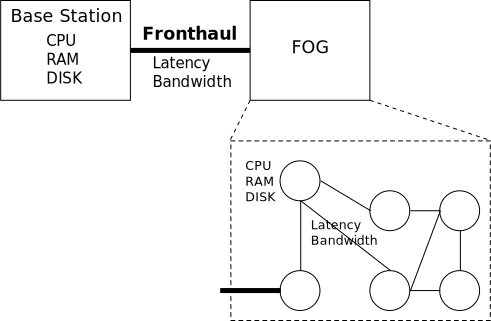
\includegraphics[width=.7\textwidth]{./images/infra.pdf}
  \caption{Fog-RAN infrastructure}
  \label{fig:infra}
\end{center}
\end{figure}

%---------------------------------------------------------
\section{Placement Problem}
%---------------------------------------------------------
A research difficulty associated to the Fog-RAN vision is where to place network functions of the BBU onto the distributed infrastructure such that functions requirements regarding CPU, RAM, latency etc. are respected and such that the overall cost is minimized. Current Cloud-RAN solutions place all BBUs functions onto the centralized Cloud.

%---------------------------------------------------------
\subsection{Split-based Placement Problem}
%---------------------------------------------------------
The first solution is based on 7 possible splits of BBU functions. BBU functions are organized into seven different categories: RF, L1-low, L1-high, L2-low, L2-high, L3-low, L3-high. A split is composed of two sides, one side will be placed onto the RRH, the other side will be placed onto one server of the Fog infrastructure.

The seven possible splits are:
\begin{itemize}
\item RRH: RF - BBU: L1/L2/L3
\item RRH: RF/L1-low - BBU: L1-high/L2/L3
\item RRH: RF/L1 - BBU: L2/L3
\item RRH: RF/L1/L2-low - BBU: L2-high/L3
\item RRH: RF/L1/L2 - BBU: L3
\item RRH: RF/L1/L2/L3-low - BBU: L3-high
\item RRH: RF/L1/L2/L3 - BBU: nil
\end{itemize}

% constraints
Considering a given source (base station), the placement problem is to choose the best split and the best server on which to place BBU functions. This placement problem should take into account the following constraints:
\begin{itemize}
\item answer CPU needs for functions placed onto a Fog server;
\item answer latency constraint between functions placed at RRH and functions placed in the Fog according to the fronthaul and CN network;
\item answer the required bandwidth.
\end{itemize}

% algorithm
The algorithm could be the following
\begin{enumerate}
\item input: demand
\item compute the 7 possible splits of the demand with associated constraints (CPU, latencies, bwdth)
\item for each split solve a placement problem to select the best server on the Fog infrastructure
\item apply a final objective function to select the best solution among the seventh best solution (one for each split)
\end{enumerate}

Definition of the placement problem (3):


\begin{figure}[t]
\begin{center}
  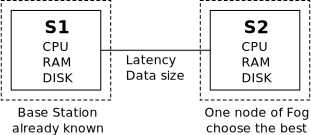
\includegraphics[width=.55\textwidth]{./images/app1.pdf}
  \caption{Split-based Fog-RAN}
  \label{fig:app1}
\end{center}
\end{figure}

%---------------------------------------------------------
\subsection{Function-based Placement Problem}
%---------------------------------------------------------
The other solution is to not limit the placement to only two sides (\ie RRH and BBUs) but to consider each function to place separately, which is closer to a usual placement problem.

In this case you will have to consider two input graphs. The first one represents the infrastructure topology (like in the first case), with nodes representing servers and links representing networks. The second one represent the graph of dependencies between BBUs functions and their associated CPU, latencies and bandwidth requirements.

\begin{figure}[t]
\begin{center}
  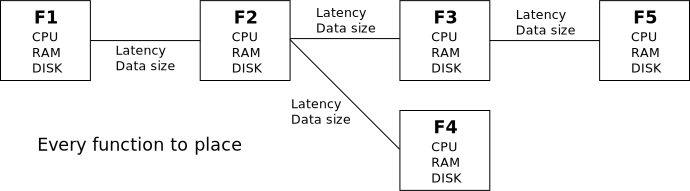
\includegraphics[width=\textwidth]{./images/app2.pdf}
  \caption{Function-based Fog-RAN}
  \label{fig:app2}
\end{center}
\end{figure}

%---------------------------------------------------------
\section{Related Work}
%---------------------------------------------------------

Paper~\cite{7371709} presents NACER, a network-aware cost efficient resource allocation method for
processing-intensive tasks in distributed Clouds. In the context of a distributed small DCs, this paper modelized a placement problem to answer VM requirements while minimizing inter-DCs communication costs. An advanced greedy algorithm is build by using the A* search algrotihm borrowed from Artificial Intelligence. Results are simulated inside CloudSIM and show very interesting results compared to simple greedy and random algorithms. It also offers an interesting state of the art analysis of other papers already read~\cite{Alicherry2012NetworkAR,6566850,7872914}. Most of them are using greedy algorithms.

None of the read paper address latencies as a strict constraint to respect~\cite{Alicherry2012NetworkAR,6566850,5662521,Steiner:2012:NSP:2377677.2377687,5461930,7872914}. All of them study the minimization of the communication cost (which is non linear and NP-hard). Handled constraints respect processing or memory requirements (linear formulation).

\cite{6217419} present a SLA-based optimization of Power and Migration Cost in Cloud Computing. The interesting part of the paper concerning our work is the model of performances, which is directly linked to latencies and response time. the response time follow an exponential distribution and time response are guaranteed in most cases with an additional penalty cost when the latency is exceeded.

\cite{silvaeuropar} present a very interesting work that takes into account latency constraints. The work modelise the network topology and the component-based application by adding a connection quality concept that reflects latencies. The network topology is modelized as a tree where leaves represents VM types or physical machines, and where inner nodes represents connections between leaves at different levels of the tree. The number of inner nodes (hops) to pass to communicate with another VM or machine thus represents the connection quality or latency. On the other hand the same connection quality is used to indicate required communication quality expected between two components of the application. Authors both consider usual bin-packing problem (requirements on capacities and cost minimization) while also taking into account communication constraints. The presented heuristics is based on a divide-and-conquer mechanism to be scalable. It first decompose the problem into sub-problems and then compose solutions to build the final placement. Papers cited that have to be read are~\cite{6253484,6256562,6495451,5461930}.

to read~\cite{Meng:2010:ERP:1809049.1809052}

%---------------------------------------------------------
\section{Discussion}
%---------------------------------------------------------
\paragraph{Split Constraints.} As BBUs functions are very well known, mathematical models exists to determine, from a given split, the expected latency between the two sides of the split, as well as CPU and RAM needed for the set of BBU functions placed onto a cloud infrastructure.
\HC{Ilhem j'aimerais avoir des d�tails sur ces mod�les}

\paragraph{Latency Constraints} Guaranteeing a latency is very difficult as it is traffic-dependent. Latencies can be more or less predicted if the network-usage is perfectly known and controlled, however, in such case the network is private and the elasticity is reduced (as in HPC clusters, private Clouds or private servers). Static models can be defined but they will not reflect reality but an approximation of the reality like in~\cite{silvaeuropar}. Dynamic models would probably be more realistic but costly (migrations, computations on the fly etc.). Another possibility is to approximate the reality but to introduce penalties when latencies are not respected. In such case, answering expected latencies is not guaranteed, as a constraint, but is included into cost minimization objectives.


\bibliographystyle{plain}
\bibliography{fogran}


\end{document}


